% Master thesis main document
% Author: Tea B.
% Revision: Ilya K.
% -------------------------------------------------------------
% ---- DOCUMENT INITIALIZATION AND PACKAGE IMPORTS
% -------------------------------------------------------------
\documentclass[12pt, twoside, openright]{book} %openany for report

\usepackage[utf8]{inputenc}				% UTF-8 input
\usepackage[english]{babel}				% Set language to english
\usepackage{blindtext}					% Use \Blinddocument or \blindmathpaper
\usepackage{graphicx}					% For graphics
\usepackage{fancyhdr}					% Fancy headers
\usepackage[hidelinks]{hyperref}		% Internal and external hyperlinks
\usepackage{amsmath}					% Math from AMS
\usepackage{amsfonts}					% Fonts from AMS
\usepackage{amsthm}						% Theorems
\usepackage{amssymb}					% Symbols
\usepackage{enumitem}					% Enumeration
\usepackage{mathtools} 					% Bonus
\usepackage{color}						% Colors
\usepackage{booktabs}					% Professional tables
\usepackage{pdfpages}					% To include PDFs
\usepackage{parskip}					% Paragraph space
\usepackage{multicol}					% For multiple columns
\usepackage[sharp]{easylist}			% For easy lists
\usepackage{makeidx}					% For the index
\usepackage[linesnumbered,ruled]{algorithm2e}	% For algorithms
\usepackage{tikz-cd}					% For diagrams
\usepackage{listings}					% To include Python-code
\usepackage{etoolbox}					% To add symbol at end of examples
\usepackage[expansion=false]{microtype} % Fixes to make typography better
\usepackage[toc, page]{appendix} 		% To include appendices
\usepackage[headings]{fullpage}		    % Smaller margins
%\usepackage[margin = 3cm, includehead, includefoot]{geometry}
\usepackage[sc]{mathpazo}				% A nice font, alternative to CM
\usepackage{framed}						% To frame comments
\usepackage{multirow}					% For multiple rows in tables
\usepackage{afterpage}					% To insert blank pages
\usepackage{blindtext}					% To insert some blind text
\usepackage{multirow}
\usepackage{amsmath}
\usepackage{graphicx}
\usepackage{textcomp}
%\usepackage{geometry}
\usepackage{floatrow}
\usepackage{layout}
\usepackage{float}
\usepackage{subfig}
\usepackage{textgreek}
\usepackage{csquotes}
\usepackage{float}
\usepackage{subfig}
\usepackage{breqn}
\usepackage{multirow}
\usepackage{gensymb}
\usepackage{listings}
\usepackage{color}
\usepackage{titlesec} 
\usepackage{caption}
\usepackage{chemscheme}
\usepackage{wrapfig}
\usepackage{notoccite}                  %citation in order of appearance
\usepackage{glossaries}
\usepackage{glossary-mcols}
\makenoidxglossaries
\floatstyle{plaintop}
\restylefloat{table}
\usepackage{lipsum}                     % Generate dummy text 
\usepackage{lineno}                     % Adds line numbers
\usepackage{graphicx}                   % For tables
\usepackage[table]{xcolor}              % For tables color
\usepackage{chngpage}                   % For changing page width for tables


\usepackage[a4paper,%
            left=3cm,right=2.5cm,top=2.5cm,bottom=2.5cm,%
            includehead, includefoot]{geometry}

\linenumbers %REMEMBER TO COMMENT OUT FOR FINAL VERSION!!!


\definecolor{mygreen}{rgb}{0,0.6,0}
\definecolor{mygray}{rgb}{0.5,0.5,0.5}
\definecolor{mymauve}{rgb}{0.58,0,0.82}
\definecolor{tabledarkgray}{HTML}{CFCFCF}
\definecolor{tablelightgray}{HTML}{E6E6E6}
% Define colours for tables, fonts, anything here! Much easier to change later 

\lstset{ 
  backgroundcolor=\color{white},   % choose the background color; you must add \usepackage{color} or \usepackage{xcolor}; should come as last argument
 % basicstyle=\footnotesize,        % the size of the fonts that are used for the code
  breakatwhitespace=false,         % sets if automatic breaks should only happen at whitespace
  breaklines=true,                 % sets automatic line breaking
  %captionpos=b,                    % sets the caption-position to bottom
  commentstyle=\color{mygreen},    % comment style
  deletekeywords={...},            % if you want to delete keywords from the given language
  escapeinside={\%*}{*)},          % if you want to add LaTeX within your code
  extendedchars=true,              % lets you use non-ASCII characters; for 8-bits encodings only, does not work with UTF-8
  %firstnumber=1000,                % start line enumeration with line 1000
  %frame=single,	                   % adds a frame around the code
  keepspaces=true,                 % keeps spaces in text, useful for keeping indentation of code (possibly needs columns=flexible)
  keywordstyle=\color{blue},       % keyword style
  language=Python,                 % the language of the code
  morekeywords={*,...},            % if you want to add more keywords to the set
  numbers=left,                    % where to put the line-numbers; possible values are (none, left, right)
  numbersep=5pt,                   % how far the line-numbers are from the code
  numberstyle=\tiny\color{mygray}, % the style that is used for the line-numbers
  rulecolor=\color{black},         % if not set, the frame-color may be changed on line-breaks within not-black text (e.g. comments (green here))
  showspaces=false,                % show spaces everywhere adding particular underscores; it overrides 'showstringspaces'
  showstringspaces=false,          % underline spaces within strings only
  showtabs=false,                  % show tabs within strings adding particular underscores
  stepnumber=2,                    % the step between two line-numbers. If it's 1, each line will be numbered
  stringstyle=\color{mymauve},     % string literal style
  tabsize=2,	                   % sets default tabsize to 2 spaces
  %title=\lstname                   % show the filename of files included with \lstinputlisting; also try caption instead of title
}

% Set up for code listings I use - Ilya
% If you use this one, comment out line 25-52
\lstdefinestyle{my_style}{
    basicstyle=\ttfamily\footnotesize,                              
    numbers=left,
    stepnumber=1,  
    breaklines=true,                % sets automatic line breaking                               
    showspaces=false,                
    showstringspaces=false,
    showtabs=false,                  
    frame=single,
    rulecolor=\color{gray},
    stringstyle=\color{mymauve},     % string literal style
    numberstyle=\tiny\color{mygray}, % the style that is used for the line-numbers
    commentstyle=\color{mygreen},    % comment style
    keywordstyle=\color{blue}        % keyword style
}
\lstset{style=my_style}








% -------------------------------------------------------------
% ---- PACKAGE SET UP
% -------------------------------------------------------------

\graphicspath{{Master/figs/}}					% Path to graphics
\pagestyle{fancy}						% Set page headers to fancy


% Add symbols at the end of example and definitions
\AtEndEnvironment{example}{\null\hfill $\lrcorner$}%
\AtEndEnvironment{definition}{\null\hfill $\lrcorner$}%

% Must run this command to use index
\makeindex

% Spacing in easylist items and rows/cols in diagrams
\newcommand{\listSpace}{-0.25em}
\newcommand{\diagramSpace}{3em}
\setlength\arrayrulewidth{1.5 pt}

% -------------------------------------------------------------
% ---- MISC SET UP
% -------------------------------------------------------------

% Include new commands
% Remember to include this in your main.tex
%% Remember to include this in your main.tex
%% Remember to include this in your main.tex
%\input{newcommands.tex} %% please check for commands here and define new commands here if needed


%--------------------------------------------------
% units
\newcommand{\GeVc}       {\ensuremath{\mathrm{GeV}/c}}
\newcommand{\GeV}        {\ensuremath{\,\mathrm{GeV}}}
\newcommand{\ns}         {\ensuremath{\,\mathrm{ns}}}
\newcommand{\us}         {\ensuremath{\,\mathrm{\upmu s}}}
\newcommand{\ms}         {\ensuremath{\,\mathrm{ms}}}
\newcommand{\nm}         {\ensuremath{\,\mathrm{nm}}}
\newcommand{\um}         {\ensuremath{\,\mathrm{\upmu m}}}
\newcommand{\mm}         {\ensuremath{\,\mathrm{mm}}}
\newcommand{\cm}         {\ensuremath{\,\mathrm{cm}}}
\newcommand{\meter}      {\ensuremath{\,\mathrm{m}}}
\newcommand{\MHz}        {\ensuremath{\,\mathrm{MHz}}}
\newcommand{\kHz}        {\ensuremath{\,\mathrm{kHz}}}
\newcommand{\Mbps}       {\ensuremath{\,\mathrm{Mbps}}}
\newcommand{\Gbps}       {\ensuremath{\,\mathrm{Gbps}}}
\newcommand{\MHzsqcm}    {\ensuremath{\,\mathrm{MHz/cm^2}}}
\newcommand{\kHzsqcm}    {\ensuremath{\,\mathrm{kHz/cm^2}}}
\newcommand{\kg}         {\ensuremath{\,\mathrm{kg}}}
% Commands for simplifying use of acronyms
\newcommand{\acf}[1]     {\acrfull{#1}}
\newcommand{\acs}[1]     {\acrshort{#1}}
\newcommand{\acl}[1]     {\acrlong{#1}}
% You can also define a word you use a lot
\newcommand{\mosaix}     {\acrshort{mosaix}}

%Usage in text 1.2~\Gbps or acs{cern} or \mosaix %% please check for commands here and define new commands here if needed


%--------------------------------------------------
% units
\newcommand{\GeVc}       {\ensuremath{\mathrm{GeV}/c}}
\newcommand{\GeV}        {\ensuremath{\,\mathrm{GeV}}}
\newcommand{\ns}         {\ensuremath{\,\mathrm{ns}}}
\newcommand{\us}         {\ensuremath{\,\mathrm{\upmu s}}}
\newcommand{\ms}         {\ensuremath{\,\mathrm{ms}}}
\newcommand{\nm}         {\ensuremath{\,\mathrm{nm}}}
\newcommand{\um}         {\ensuremath{\,\mathrm{\upmu m}}}
\newcommand{\mm}         {\ensuremath{\,\mathrm{mm}}}
\newcommand{\cm}         {\ensuremath{\,\mathrm{cm}}}
\newcommand{\meter}      {\ensuremath{\,\mathrm{m}}}
\newcommand{\MHz}        {\ensuremath{\,\mathrm{MHz}}}
\newcommand{\kHz}        {\ensuremath{\,\mathrm{kHz}}}
\newcommand{\Mbps}       {\ensuremath{\,\mathrm{Mbps}}}
\newcommand{\Gbps}       {\ensuremath{\,\mathrm{Gbps}}}
\newcommand{\MHzsqcm}    {\ensuremath{\,\mathrm{MHz/cm^2}}}
\newcommand{\kHzsqcm}    {\ensuremath{\,\mathrm{kHz/cm^2}}}
\newcommand{\kg}         {\ensuremath{\,\mathrm{kg}}}
% Commands for simplifying use of acronyms
\newcommand{\acf}[1]     {\acrfull{#1}}
\newcommand{\acs}[1]     {\acrshort{#1}}
\newcommand{\acl}[1]     {\acrlong{#1}}
% You can also define a word you use a lot
\newcommand{\mosaix}     {\acrshort{mosaix}}

%Usage in text 1.2~\Gbps or acs{cern} or \mosaix %% please check for commands here and define new commands here if needed


%--------------------------------------------------
% units
\newcommand{\GeVc}       {\ensuremath{\mathrm{GeV}/c}}
\newcommand{\GeV}        {\ensuremath{\,\mathrm{GeV}}}
\newcommand{\ns}         {\ensuremath{\,\mathrm{ns}}}
\newcommand{\us}         {\ensuremath{\,\mathrm{\upmu s}}}
\newcommand{\ms}         {\ensuremath{\,\mathrm{ms}}}
\newcommand{\nm}         {\ensuremath{\,\mathrm{nm}}}
\newcommand{\um}         {\ensuremath{\,\mathrm{\upmu m}}}
\newcommand{\mm}         {\ensuremath{\,\mathrm{mm}}}
\newcommand{\cm}         {\ensuremath{\,\mathrm{cm}}}
\newcommand{\meter}      {\ensuremath{\,\mathrm{m}}}
\newcommand{\MHz}        {\ensuremath{\,\mathrm{MHz}}}
\newcommand{\kHz}        {\ensuremath{\,\mathrm{kHz}}}
\newcommand{\Mbps}       {\ensuremath{\,\mathrm{Mbps}}}
\newcommand{\Gbps}       {\ensuremath{\,\mathrm{Gbps}}}
\newcommand{\MHzsqcm}    {\ensuremath{\,\mathrm{MHz/cm^2}}}
\newcommand{\kHzsqcm}    {\ensuremath{\,\mathrm{kHz/cm^2}}}
\newcommand{\kg}         {\ensuremath{\,\mathrm{kg}}}
% Commands for simplifying use of acronyms
\newcommand{\acf}[1]     {\acrfull{#1}}
\newcommand{\acs}[1]     {\acrshort{#1}}
\newcommand{\acl}[1]     {\acrlong{#1}}
% You can also define a word you use a lot
\newcommand{\mosaix}     {\acrshort{mosaix}}

%Usage in text 1.2~\Gbps or acs{cern} or \mosaix

% A command to add a blank page
\newcommand\blankpage{%
	\null
	\newpage}

% Header set up with fancyhdr
\lhead[\nouppercase{\leftmark}]{\thepage} % EVEN, ODD
\rhead[\thepage]{\nouppercase{\rightmark}} % EVEN, ODD
\cfoot[]{}

\pagestyle{fancy}
\fancypagestyle{normal}{%
	% Header set up with fancyhdr
	\lhead[\nouppercase{\leftmark}]{\thepage} % EVEN, ODD
	\rhead[\thepage]{\nouppercase{\rightmark}} % EVEN, ODD
	\cfoot[]{}}
\fancypagestyle{noheadername}{%
	% Header set up with fancyhdr
	\lhead[]{\thepage} % EVEN, ODD
	\rhead[\thepage]{} % EVEN, ODD
	\cfoot[]{}}

% Declare first page in every chapter as 'fancy' pagestyle
\makeatletter
\renewcommand\chapter{\if@openright\cleardoublepage\else\clearpage\fi
	\thispagestyle{fancy}%
	\global\@topnum\z@
	\@afterindentfalse
	\secdef\@chapter\@schapter}
%\makeatother\setlength\bibitemsep{0.9\baselineskip}

% Custom environment for comments
\newenvironment{comment}{\begin{framed} \footnotesize \textcolor{red}{\textbf{Comment.}}}{\end{framed} \normalsize}

% Set up for Acronyms
%Alternative approach

%\begin{acronym}
%    \acro{CERN}{\emph{European Organization for Nuclear Research}}
%\end{acronym}

%examples of how to use acronyms in the main text
%\ac{ADC} = Analog to Digital Converter (ADC)
%\acs{ADC} = ADC
%\acsp{ADC} = ADCs

\newacronym{tc}{TC}{Transition Card}
\newacronym{pcu}{PCU}{Power Control Unit}
\newacronym{pru}{pRU}{pCT Readout Unit}
\newacronym{psu}{PSU}{Power Supply Unit}
\newacronym{pct}{pCT}{proton Computed Tomography}
\newacronym{uib}{UiB}{University of Bergen}
\newacronym{alpide}{ALPIDE}{ALICE Pixel Detector}
\newacronym{alice}{ALICE}{A Large Ion Collider Experiment}
\newacronym{ct}{CT}{Computed Tomography}
\newacronym{dtc}{DTC}{Digital Tracking Calorimeter}
\newacronym{pcb}{PCB}{Printed Circuit Board}
\newacronym{lhc}{LHC}{Large Hadron Collider}
\newacronym{lvds}{LVDS}{Low-Voltage Differential Signaling}
\newacronym{cern}{CERN}{European Organization for Nuclear Research}
\newacronym{its}{ITS}{Inner Tracking System}
\newacronym{gui}{GUI}{Graphical User Interface}
\newacronym{mvc}{MVC}{Model-View-Controller}
\newacronym{visa}{VISA}{Virtual Instrument Software Architecture}
\newacronym{usb}{USB}{Universal Serial Bus}
\newacronym{gpib}{GPIB}{General Purpose Interface Bus}
\newacronym{rs232}{RS-232}{Recommended Standard 232, serial communication transmission of data}
\newacronym{centos}{CentOS}{Community Enterprise Operating System}
\newacronym{cmos}{CMOS}{Complementary Metal Oxide Semiconductor}
\newacronym{sobp}{SOBP}{Spread-Out Bragg Peak}
\newacronym{let}{LET}{Linear Energy Transfer}
\newacronym{fpga}{FPGA}{Field Programmable Gate Array}
\newacronym{dch}{DCH}{Direct Connect System}
\newacronym{ff}{FF}{FireFly}
\newacronym{fpc}{FPC}{Flexible Printed Circuit}
\newacronym{rcu2}{RCU2}{Readout Control Unit Version 2}
\newacronym{zif}{ZIF}{Zero Insertion Force}
\newacronym{ipc}{IPC}{Institute of Printed Circuit}
\newacronym{emi}{EMI}{Electromagnetic Interference}
\newacronym{dtu}{DTU}{Data Transmission Unit}
\newacronym{pll}{PLL}{Phase Locked Loop}
\newacronym{dut}{DUT}{Device Under Test}
\newacronym{prbs}{PRBS}{Pseudorandom Binary Sequence}
\newacronym{esd}{ESD}{Electrostatic Discharge}
\newacronym{ic}{IC}{Integrated Circuit}
\newacronym{idc}{IDC}{Insulation-Displacement Connector}
\newacronym{pla}{PLA}{Polylactic Acid}
\newacronym{bom}{BOM}{Bill of Materials}
\newacronym{daq}{DAQ}{Data Acquisition}
\newacronym{tid}{TID}{Total Ionizing Dose}
\newacronym{maps}{MAPS}{Monolithic Active Pixel Sensor}
\newacronym{udp}{UDP}{User Datagram Protocol }
\newacronym{sram}{SRAM}{Static Random Access Memory}
\newacronym{mlvds}{MLVDS}{Multipoint \acrlong{lvds}}
\newacronym{i2c}{I2C}{Inter-Integrated Circuit}
\newacronym{spi}{SPI}{Serial Peripheral Interface} 
\newacronym{rtd}{RTD}{Resistance Temperature Detector}
\newacronym{phy}{PHY}{Physical Layer}
\newacronym{mac}{MAC}{Media Access Control}
\newacronym{ptb}{PTB}{Production Test Box}
\newacronym{mpsoc}{MPSoC}{Multiprocessor System on a Chip}
\newacronym{ups}{UPS}{Uninterruptible Power Supply}
\newacronym{rcbo}{RCBO}{Residual-Current Circuit Breaker with Overcurrent Protection}


% Set up for chapter title style
\titleformat{\chapter}[display]
  {\mdseries\large}
  {\filleft\MakeUppercase{\chaptertitlename} \large\thechapter}
  {1ex}
  {\titlerule\vspace{2ex}\filright\Huge}
  [\vspace{2ex}\titlerule]

\setlength{\headheight}{14.5pt} % Set to 14.5pt to remove warning


\begin{document}
	
	% ---------------------------------------------------------
	% ---- Title page
	% ---------------------------------------------------------
	
	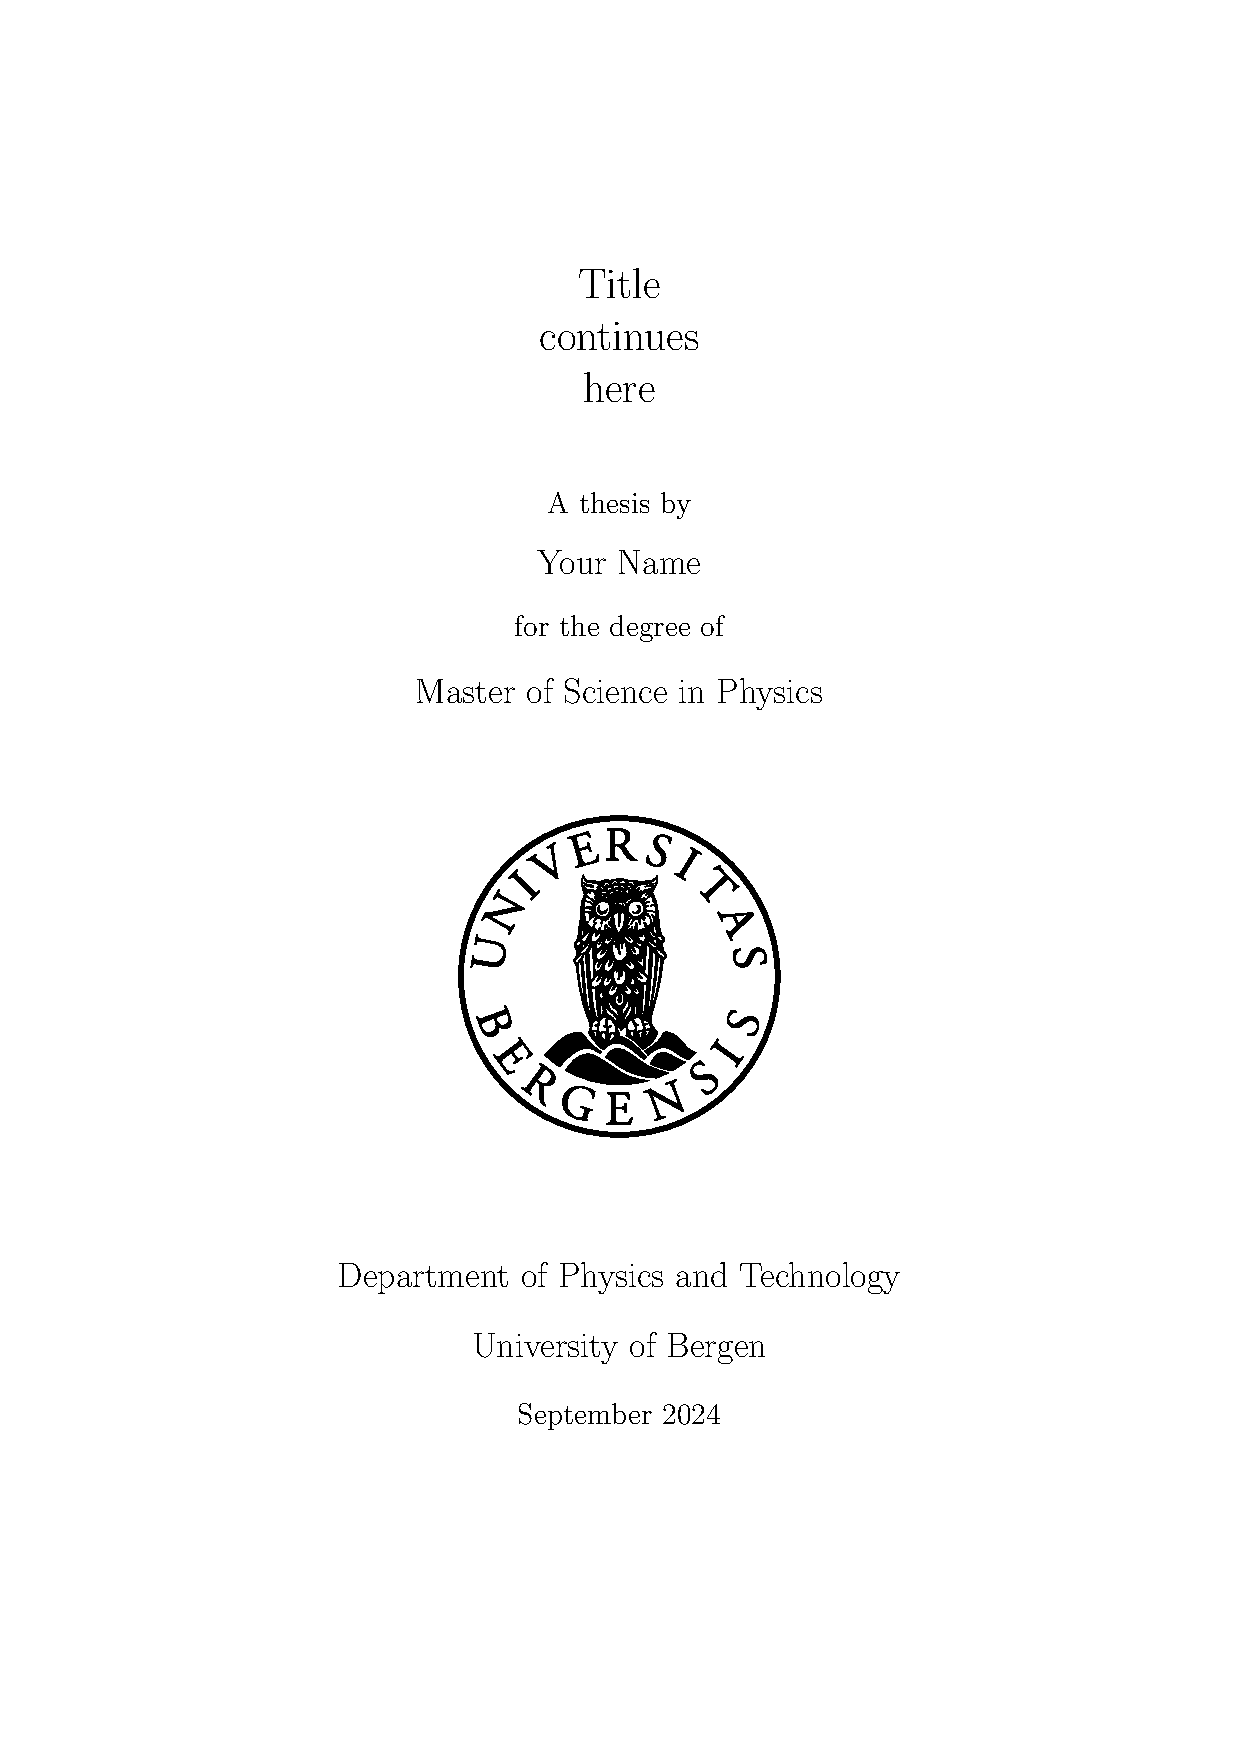
\includepdf{cover/cover.pdf} %The pdf must be generated separately to avoid unwanted changes from the main 
	\pagestyle{empty}
	\afterpage{\blankpage}
	\clearpage
	
	% ---------------------------------------------------------
	% ---- DOCUMENT INTRODUCTION
	% ---------------------------------------------------------
	

	\pagenumbering{roman}
   
    \chapter*{Abstract}
    \addcontentsline{toc}{chapter}{Abstract}
    
\lipsum[2-3]

% Write at the very end or when you have written intro and conclusion
    \clearpage
    
    
    \chapter*{Acknowledgments}
    \addcontentsline{toc}{chapter}{Acknowledgements}
    
\lipsum[2-3]

% Allowed to be more relaxed






    \clearpage

    \chapter*{Generative AI Declaration}
    \addcontentsline{toc}{chapter}{Generative AI Declaration}
    
Generative artificial intelligence (AI) has been used in this thesis.
As the author, I am fully responsible for the content, claims, and references.

\lipsum[2]
% Write which AI you used and how (what queries)
    \clearpage 
    
    % Now the table of contents
	\tableofcontents
	\clearpage

    \chapter*{Thesis Outline}
    \addcontentsline{toc}{chapter}{Thesis Outline}
    \textbf{Chapter 1: Introduction} \quad
\lipsum[1][1-3]

\textbf{Chapter 2: NAME} \quad
\lipsum[2][1-3]

\textbf{Chapter 3: NAME} \quad
\lipsum[3][1-3]

\textbf{Chapter 4: Summary and Conclusion} \quad
\lipsum[4][1-3]

\textbf{Appendix A: NAME} \quad
\lipsum[5][1-3]
    \clearpage
    
    % Acronyms
    \printnoidxglossary[style=mcolindex,title=Acronyms, 
    toctitle=List of terms,nonumberlist]
	\addcontentsline{toc}{chapter}{Acronyms}
	
	\listoffigures
	\addcontentsline{toc}{chapter}{List of Figures}
	\listoftables
	\addcontentsline{toc}{chapter}{List of Tables}
    \lstlistoflistings
    \addcontentsline{toc}{chapter}{List of Listings}
	\newpage
    \mbox{}
    \newpage

	
	% ---------------------------------------------------------
	% ---- MAIN PART OF DOCUMENT
	% ---------------------------------------------------------
	
	\pagenumbering{arabic}
	\pagestyle{normal}
	
	\chapter{Introduction}
        \label{chap:intro} % Use to reference chapters in text
    	
\section{Background and Motivation}
\label{sec:background} % Use for all sections and subsection for easy ref in text

This references Section \ref{sec:background}, or maybe Chapter \ref{chap:chapter}, or Appendix \ref{app:title}.

\section{About this Thesis}
\label{sec:about_thesis}

How to use acronyms:

\acrfull{cern}

\acrlong{cern}

\acrshort{cern}

\acrfull{alice}

Levels of text:

\section{Section}
\label{sec:section}

\lipsum[2][1-4]

\subsection{Subsection}
\label{sec:subsection}

\lipsum[2][1-4]

\subsubsection{Subsubsection}
% I don't usually reference subsubsections since they don't have a number in pdf

\lipsum[2][1-4]

\section{Citation Principles}
\label{sec:citation-principles}
This thesis uses the principle that citations listed after the ending punctuation of a paragraph may refer to several statements in the section. 
Citations listed before any punctuation will always refer to the last statements.

    
	\chapter{Chapter Name}
        \label{chap:chapter}
        \lipsum[2]


\section{Figures}
\label{sec:figures}

Reference to Figure \ref{fig:alice-detector}

\begin{figure}[ht]
    \centering
    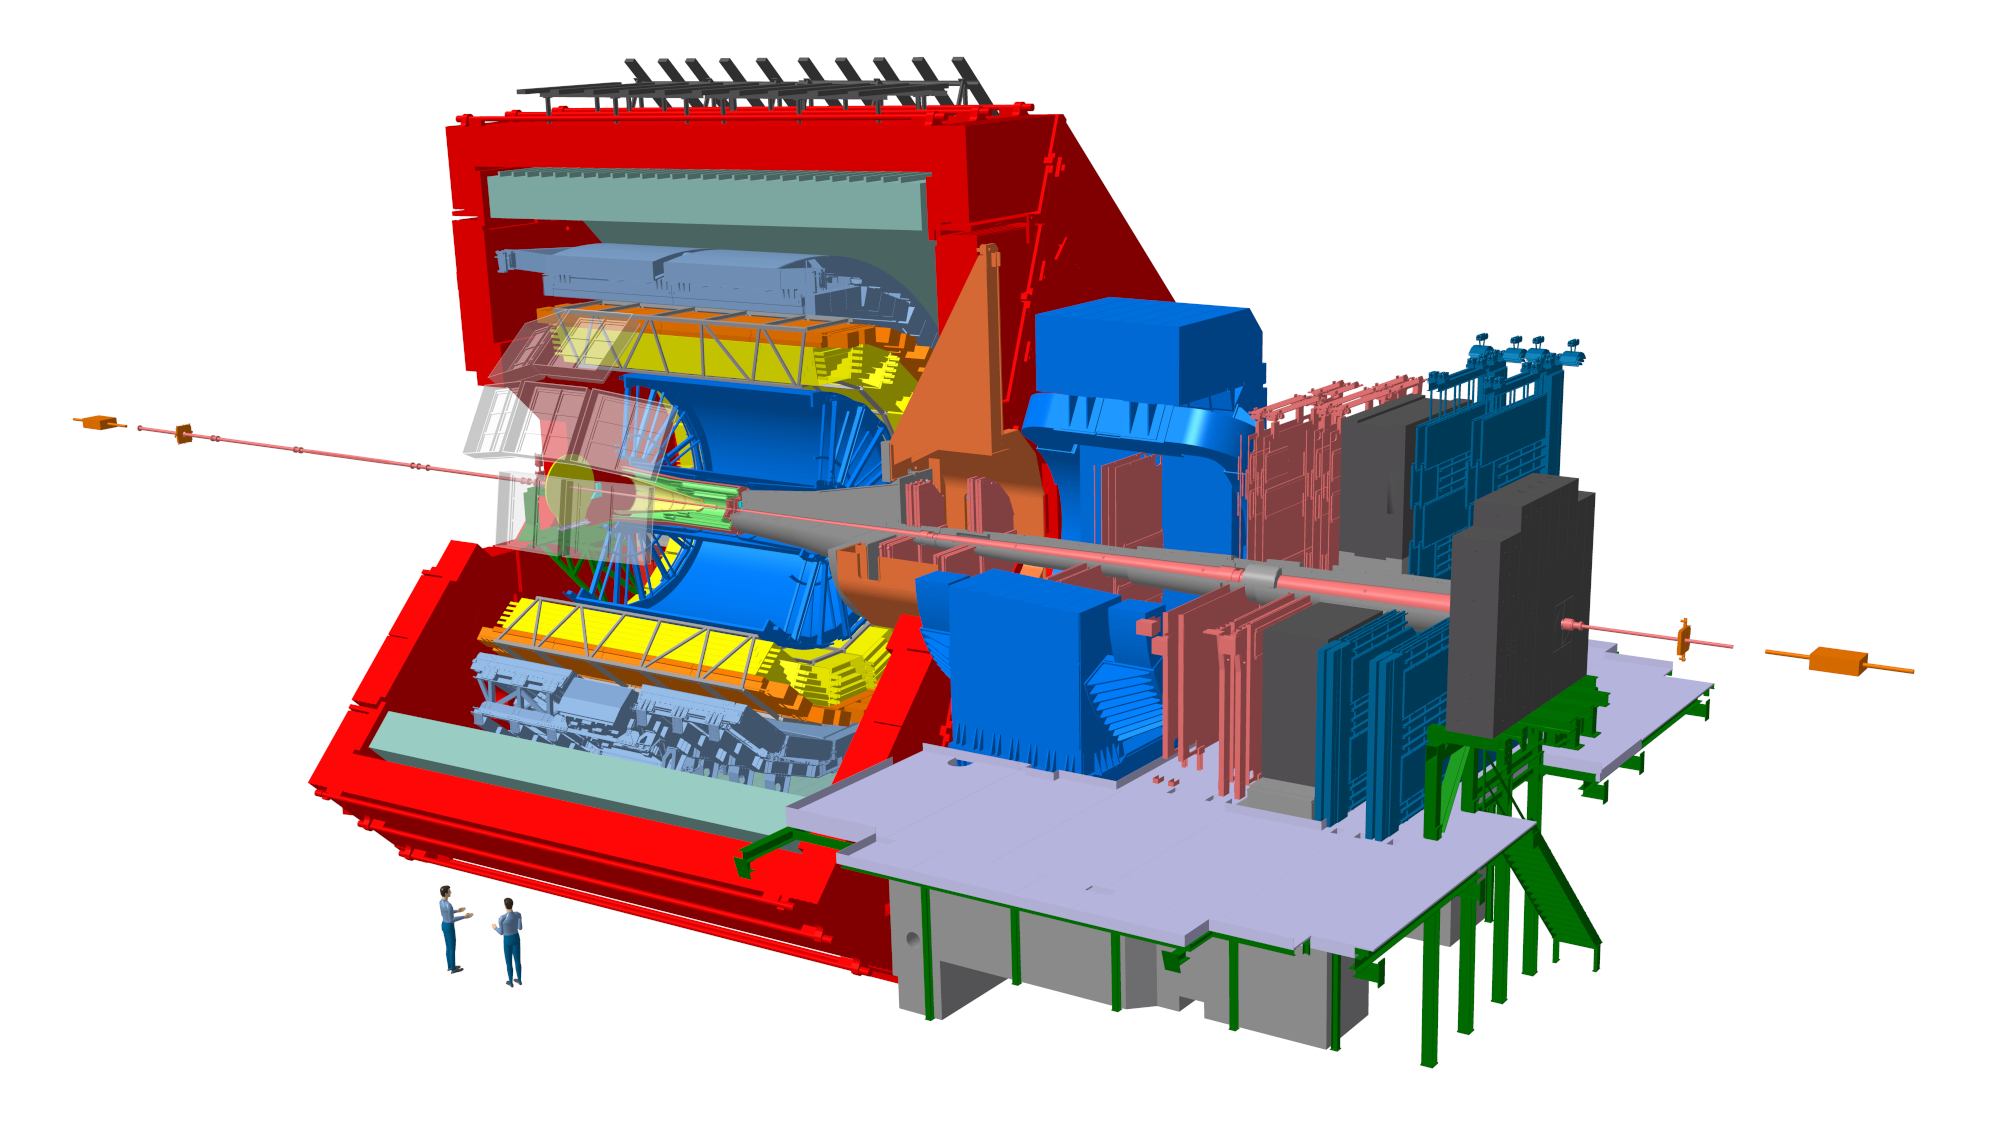
\includegraphics[width=0.8\textwidth]{Master/figs/alice_detectors.jpg}
    \caption[Figure text in list of figs]{Figure text in main text. (Remember citation)}
    \label{fig:alice-detector}
\end{figure}

\section{List}
\label{sec:list}

\begin{itemize}
    \item First
    \item Second
    \item Third
\end{itemize}

\section{Tables}
\label{sec:table}
% Use https://www.tablesgenerator.com/latex_tables#
% to generate tables, copy then into text

\begin{table}[ht]
    \centering
    \caption[Overview of clock domains]{Clock domain overview with frequencies and description.}
    \label{tab:clk-domains}
    \resizebox{\textwidth}{!}{%
    \begin{tabular}{@{}|l|r|l|@{}}
        \hline
        \rowcolor{tabledarkgray} 
                                            & \textbf{Clock Frequency} & \textbf{Description} \\ \hline
        \textbf{refclk\_i}                  & 320 \MHz{}               & \begin{tabular}[c]{@{}l@{}}Reference clock for the receivers \\ generated on the base-board\end{tabular}                    \\ \hline
        \rowcolor{tablelightgray} 
        \textbf{clk33\_i}                   & 33.3 \MHz{}              & \begin{tabular}[c]{@{}l@{}}Reference clock for the Clock Controller \\ generated by the system-on-chip\end{tabular}         \\ \hline
        \textbf{clk160\_i}                  & 160 \MHz{}               & \begin{tabular}[c]{@{}l@{}}Reference clock for the Clock Controller \\ generated on the base-board\end{tabular}             \\ \hline
        \rowcolor{tablelightgray}
        \textbf{system\_clk}                & 100 \MHz{}               & \begin{tabular}[c]{@{}l@{}}Main clock for the test system\end{tabular}                                                      \\ \hline
        \textbf{data\_clk}                  & 160 \MHz{}               & \begin{tabular}[c]{@{}l@{}}Clock used for the data path\end{tabular}                                                        \\ \hline
        \rowcolor{tablelightgray}
        \textbf{slow\_control\_fast\_clk}   & 80 \MHz{}                & \begin{tabular}[c]{@{}l@{}}Clock used for Slow Control modules\end{tabular}                                                 \\ \hline
        \textbf{lhc\_clk}                   & 40 \MHz{}                & \begin{tabular}[c]{@{}l@{}}Clock used for the sync generator \\ synchronized to the frequency of the \acs{lhc}\end{tabular} \\ \hline
        \rowcolor{tablelightgray}
        \textbf{testout\_oversampling\_clk} & 640 \MHz{}               & \begin{tabular}[c]{@{}l@{}}Clock used for the testout deserializer\end{tabular}                                            \\ \hline
    \end{tabular}%
    }
\end{table}

\section{Listings}
\label{sec:listings}

\begin{lstlisting}[
    language=Python, 
    caption={[Test bench driver definition]Test bench example: driver definition.}, 
    label=lst:tb-driver-def, 
    float=!htbp
    ]
def get_ipb(dut):
ipbus = IpBusDriver(
    dut,
    "ipbus",
    dut.ipb_clk,
    dut.ipb_in.ipb_addr,
    dut.ipb_in.ipb_wdata,
    dut.ipb_in.ipb_strobe,
    dut.ipb_in.ipb_write,
    dut.ipb_out.ipb_rdata,
    dut.ipb_out.ipb_ack,
    dut.ipb_out.ipb_err,
)
return ipbus
\end{lstlisting}

\section{Citation}
\label{sec:citation}

Citations referencing this statement come before punctuation \cite{safety}. 
Citations referencing the whole paragraph come at the very end of the paragraph, after punctuation. \cite{aluminium_LUT}

\section{Footnotes}
\label{sec:foot}

This is how you use a footnote\footnote{This is a footnote.}.
	
	\chapter{Summary and Conclusion}
        \label{chap:outro}
        
\section{Summary}


\section{Future Work}


\section{Conclusion}

        \newpage

	% ---------------------------------------------------------
	% ---- APPENDICES
	% ---------------------------------------------------------
	
	\begin{appendices}
    
        \chapter{Title}
            \label{app:title}
            \lipsum[2-4]
     
	\end{appendices}
	

	
	
	% ---------------------------------------------------------
	% ---- BIBLIOGRAPHY
	% ---------------------------------------------------------
   \cleardoublepage{}\phantomsection\addcontentsline{toc}{chapter}{Bibliography}
    \bibliography{final} % Name of the .bib file in use
    \bibliographystyle{IEEEtran}
    %\nocite{*} %prints all references
\end{document}

